%\subsection{Image Formation}
\label{chapter:imform}

%The gigapixel implementation of QIS is still in the proposal phase. The current prototypes of the quanta imaging sensors incorporate around 10Mjots. However, the concept of the image reconstruction following the initial readout of the sensor data does not indicate any possible complications through scaling of the array dimensions; the principles employed during post-processing are governed by the same physical processes and presume the sources of error of the same magnitude.

The image formation process in a QIS imaging sensor consists of two fundamental processing blocks and can be seen in Figure \ref{fig:qismodel}. For reasons of simplicity, we present the model based on the single-bit sensor.

\begin{figure}[h]
  \centering
  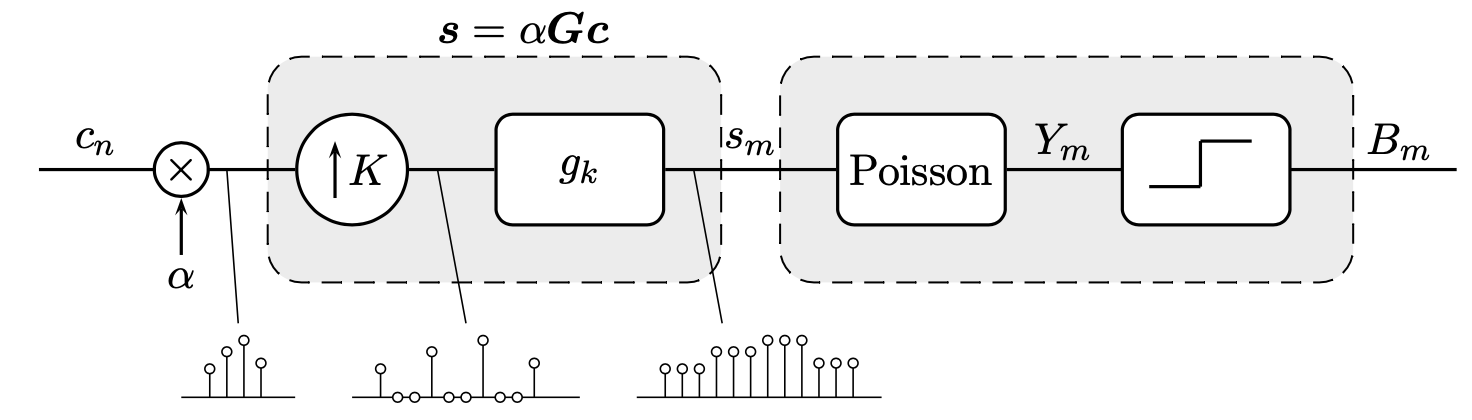
\includegraphics[width=\linewidth]{imgs/qis/qis-model.png}
  \caption{QIS image formation model, via \cite{s16111961}.}
  \label{fig:qismodel}
  \Description{The image reconstruction model for QIS applications.}
\end{figure}

The first block comprises operations necessary to perform spatial oversampling of the diffraction-limited light field. In the second block, the upsampled light undergoes the binary sensing, where the exposure values are filled in using the one-bit quantized Poisson statistics.

It should be noted that the temporal oversampling is omitted in this particular figure, though it is foreseen by definition.

\subsection{Spatial Oversampling of the Light Field}

Assuming $N$ discrete spatial coordinates, i.e. the amount of observable pixels per unit space, the light intensities are a vector of coefficients in discrete space $\boldsymbol{c}=\left[c_{0}, \ldots, c_{N-1}\right]^{T}$. For convenience, we consider the variables to be acquired in a one-dimensional space, i.e., a vector $\boldsymbol{c}_{N \times 1}$. 

The signal is assumed to be normalized to prevent scaling ambiguity such that $c_n \in [0,1]$. In order to achieve the proper range scaling for the observations, the inputs are upscaled via multiplication with the factor $\alpha > 0$, representing the \textit{sensor gain}. Afterwards, the existing data is ready to be spatially upsampled with the specified degrees of freedom needed for the modelling. 

Depending on the total amount of jots $M$, every observation $c_n$ is multiplied by the \textit{spatial oversampling factor} $ K \stackrel{\Delta}{=} \frac{M}{N} $; every diffraction-limited pixel is subsequently spread out outwards. It is per definition that the $K \in \mathbb{Z}^{+} $.

The missing intensity values are filled in via lowpass filtering with a discrete, non-negative kernel $\boldsymbol{g}$; a common choice for an interpolation kernel is the box-car function, which is defined such that it's coefficients are
\begin{equation}g_k = \frac{1}{k} \;\textup{for} \;k = 0, 1, ... , K-1.\end{equation}

Although other lowpass filtering operators are available (\cite{Feng_Yang_2012} name cardinal B-splines and squared sinc function), boxcar function is assumed to be the most accurate emulation of the oversampled light field: due to the microlenticular lenses placed in front of the jots in most functioning prototypes, it can be safely assumed that the light is focused on each jot.\cite{qisthreshold}

Assuming the sampling is performed using the box\-car filtering function, one can describe the entirety of the oversampling process as a sequence of linear operations; the aforementioned operations can therefore be concatenated und rewritten in the form of $\boldsymbol{s} = \alpha \boldsymbol{G}_c $, corresponding to a matrix-vector multiplication with the filter response function $\boldsymbol{G}_c$ of the interpolation filter in the Fourier domain.

\begin{figure}[h]
  \centering
  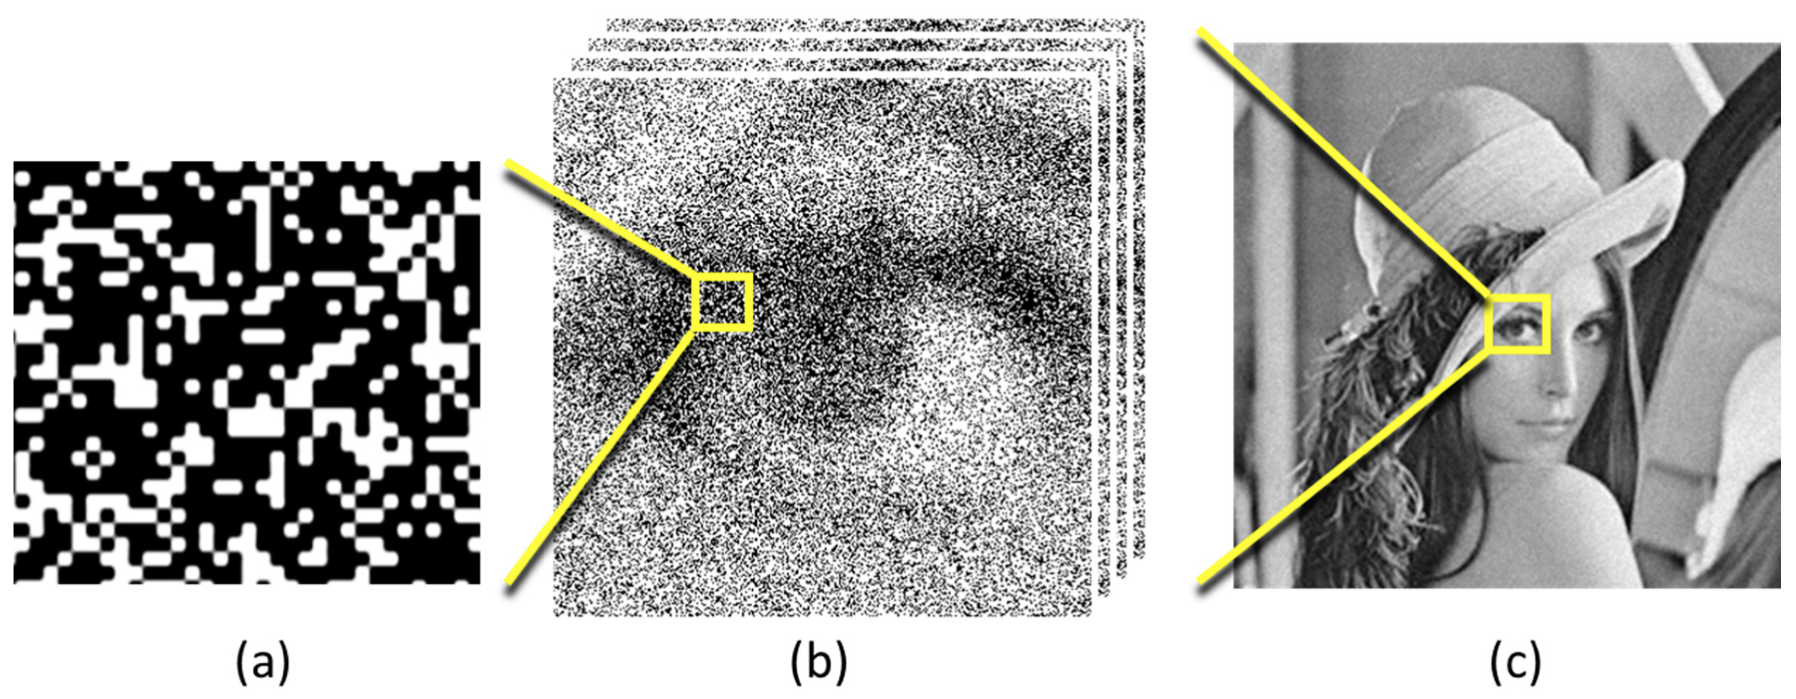
\includegraphics[width=0.8\linewidth]{imgs/qis/jotdatasimulation.png}
  \caption{Oversampled light field simulation. Via: \cite{fossum2016quanta}}
  \label{fig:jotdata}
  \Description{The common image of Lenna has film-like qualities due to being oversampled using Poisson statistics.}
\end{figure}

\subsection{Binary Sensing}

The oversampled light field, already provided in discrete form, has to be approximated further by simulating the light fluctuation throughout the jot device and the subsequent thresholding. 

The fluctuations, i.e. the photon shot noise, adhere to the Poisson distribution. In measurements over an arbitrary period of time $t$, the probability of obtaining $y_{m}$ photoelectrons is based on exposure $s_{m}$ like
\begin{equation}\mathbb{P}\left\{Y_{m}=y_{m} ; s_{m}\right\}=\frac{s_{m}^{y_{m}} e^{-s_{m}}}{y_{m} !}\end{equation}

%\begin{equation}\mathbb{P}\left\{k\right\}=\frac{e^{-H}H^{k}}{k !}.\end{equation}
%$\mathbb{P}\left\{B_{m}=1 ; s_{m}\right\}=\mathbb{P}\left\{Y_{m} \geq q ; s_{m}\right\}=\sum_{k=q}^{\infty} \frac{s_{m}^{k} e^{-s_{m}}}{k !}$
The quantization process is a mapping of detected photoelectrons into the binary range, based on the non-negative threshold $q$: $B: \mathbb{Z}^{+} \cup\{0\} \longmapsto\{0,1\}$.

\begin{equation}\boldsymbol{B}(y) \stackrel{ \Delta }{=}\left\{\begin{array}{ll}1 & \text { for } y \geq q \\ 0 & \text { otherwise }\end{array}\right.\end{equation}

For a threshold of $q = 1$, the probabilities of no photon arrivals are therefore estimated as 
\begin{equation}\label{eq:poisson0}\quad \mathbb{P}\left\{B_{m}=0 ; s_{m}\right\}=e^{-s_{m}} \quad\end{equation}leaving us with $\mathbb{P}\left\{B_{m}=1 ; s_{m}\right\}=1-e^{-s_{m}}$ otherwise.

%\subsubsection{Non-Linearity and the Bit Density}
%\label{chapter:nlbd}
%\cite{FossumSiMulQIS} manages to relate the probabilities of detection to the sensitivity response of QIS, and does so on a larger scale, observing clusters of multiple jots.

%In a single-bit photon-counting sensor, the probability of no arrivals is given via Equation \ref{eq:poisson0}. For $M$ uniformly illuminated jots, the number of jots with such state is $M \times e^{-s_{m}}$, or $M \times e^{-H}$; remaining jots with the response of 1 are $M \times (1- e^{-H})$, accordingly.

\subsection{Error Rates}
In the presented model, only natural photon shot noise is considered~\cite{Feng_Yang_2012, s16111961}. Generally, the signal transfer chain is much closer to the equation

\begin{equation}\boldsymbol{x}_{\mathrm{QIS}}=\operatorname{ADC}\{\text { Poisson }(\alpha \cdot \boldsymbol{x}_{\text {true}}+\boldsymbol{\eta}_{\mathrm{dark}}))+\boldsymbol{\eta}_{\mathrm{read}}\}\end{equation}

and the photon noise is less dominant under sparse exposures. 

Generally, there is also read noise, introduced by the readout process through the readout circuit transistors (resulting in flicker noise, 1/f) and reset on capacitors. These are critical in low-light imaging conditions, where the number of photoelectrons is sparse. The readout noise is often referred to the equivalent number of input photoelectrons.\cite{7422662}. 

In a normalized uncorrupted signal \begin{equation}
U_{s i g} \triangleq \frac{V_{s i g}}{C G}
\end{equation}
the value is only dependant on the number of photoelectrons readout, i.e. the \textit{electron number}, and is Poisson distributed. There is equivalence between the interpretation of the electron number and the ratio of the voltage to conversion gain $CG$.

However, assuming additional read noise, normalized as
\begin{equation}
    u_{n} \triangleq \frac{v_{n}}{C G}
\end{equation}

the probability distribution function depends not just on obtaining a certain amount of photoelectrons, but the noise $u_{n}$ as well. Since the read noise is best approximated through Gaussian, the total probability is a convolution of the Poisson distribution for quanta exposure H (equivalent to $s_m$ in previous chapters) and a normal distribution with read noise $u_n$. 

\begin{equation}\mathbb{P}[U]=\sum_{k=0}^{\infty} \frac{\mathbb{P}[k]}{\sqrt{2 \pi u_{n}^{2}}} \exp \left[-\frac{(U-k)^{2}}{2 u_{n}^{2}}\right]
\end{equation}

When $U_{sig}$ is quantized with a 1b analog-to-digital-converter, it is subjected to a comparison with a threshold $U_{th}$, commonly 0.5~\cite{FossumSiMulQIS}. With fluctuations caused by read noise, the binary response is prone to errors. 
We are presented with two options: either there are no electrons, but the 0 is misquantized as 1 due to the added noise, or there is a positive response of 1 misquantized as 0. The sum of these false positives and false negatives in ratio to total number of jots is the \textit{Bit Error Rate} (BER).

\begin{figure}[h]
  \centering
  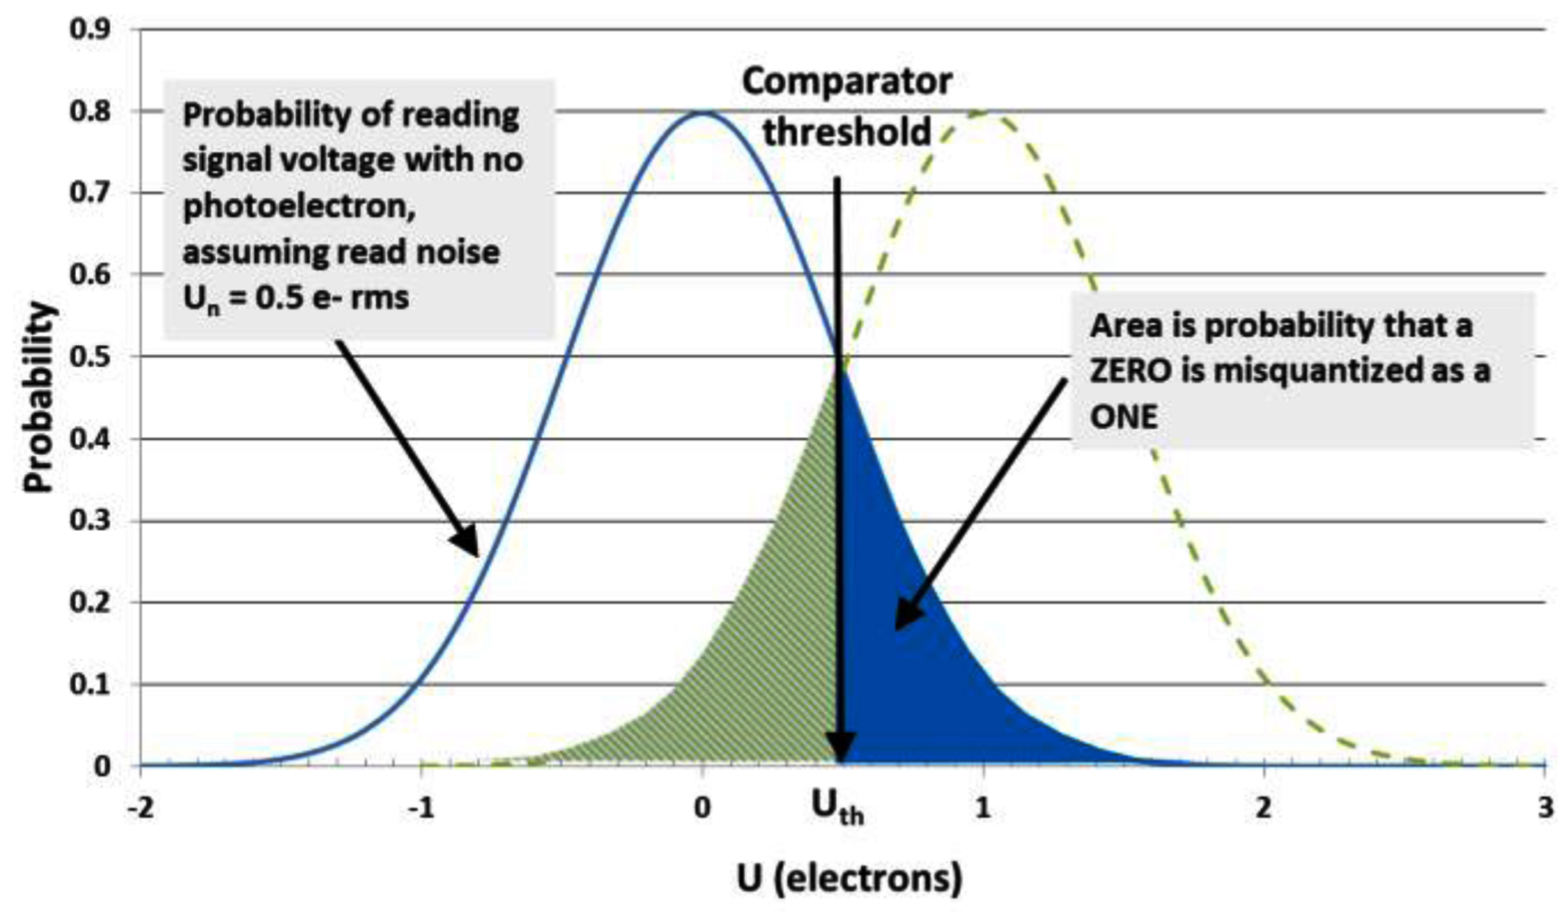
\includegraphics[width=0.8\linewidth]{imgs/ber.png}
  \caption{Bit Error Rate in single-bit sensors, via \cite{FossumSiMulQIS}.}
  \label{fig:berrate}
  \Description{Two parabolic functions with overlaps in the middle of the chart. The overlap characterizes the erroneous measurements}
\end{figure}

In Figure \ref{fig:berrate}, the misquantizations are shown for the single-bit case with a threshold exactly in the middle. There are only two possible states, and for each state, there's a possibility of an error. The false estimations are formed in the overlapping section.

The false negatives and false positives are obtained through the integration of the probability distribution function,
which leads us to expressing these as an error function:

\begin{equation}
    P_{f n}=\frac{1}{2} \operatorname{erfc}\left[\frac{1-U_{t h}}{\sqrt{2} U_{n}}\right]
\end{equation}
and
\begin{equation}
P_{f p}=\frac{1}{2} \operatorname{erfc}\left[\frac{1}{\sqrt{8} U_{n}}\right]
\end{equation}

When the threshold is put exactly in the middle, the false positives and false negatives are equally probable. The total bit error rate with the threshold of $U_{th}=0.5$ amounts to 

\begin{equation}
B E R=\frac{1}{2} \operatorname{erfc}\left[\frac{1}{\sqrt{8} U_{n}}\right]\end{equation}

and is only acceptably small with read noise of 0.30$e^{-}$ r.m.s. and below.
